%======================================================================
\chapter{Measuring Renyi Entanglement Entropy}
%======================================================================
\comment{Totally why do we measure this?  Y'know?}\\
\comment{Mention we're using double projector}

\noindent
- we can't measure \vn with vb qmc\\
- \vb isn't a good measure of entropy\\
- can measure \re\\
 - closest entropy to \vn\\
 - gives a lower bound on \vn\\
 - maybe follows same area law and still has universal terms? (check)\\
 
The generalized Renyi entanglement entropies, again defined as:
\begin{equation} \label{renyi2}
 	S_n(\rho_{\rm A}) = \frac{1}{1-n}\ln\left[{\rm Tr}\left( \rho_{\rm A}^n \right) \right],
\end{equation}
where $\rho_{\rm{A}}=\rm{Tr}_B\ket{\psi}\bra{\psi}$ is the reduced density matrix of region A, and $n>0$.

\change{
``Encode information about the whole entanglement spectrum of $\rho_{\rm A}$."
(But that's just because if you know all of them you pretty much know all the eigenvalues of $\rho_{\rm A}$.)
So they have more information together than just $S_1=\VN$. \cite{Spectrum}
}

\change{ Something about topological entanglement entropy and quantum dimension \cite{Bbob}.}

\change{ Field theory on $O(N)$ model... universal corrections to scaling of $S_n$ calculated.}

The Renyi entropies have the property that successive entropies give a lower bound on the previous entropies.  I.e. if $n>m$ then $S_n<S_m$, so \re gives a lower bound on \vN, and \re will give the closest estimate of \vN.

We can use the expectation value of a unitary \sw operator on two non-interacting copies of the system to be studied in order to obtain ${\rm Tr}(\rho_{\rm A}^2)$, a quantity necessary to compute \re.  
This process can be generalized to calculate any $S_n$ with $n \ge 2$, by applying a generalized \sw operator to $n$ copies of the system. 

\section{The ``Replica Trick''}
%----------------------------------------------------------------------------------------------------------
\subsection{The Swap Operator}
%----------------------------------------------------------------------------------------------------------

\begin{figure} {
	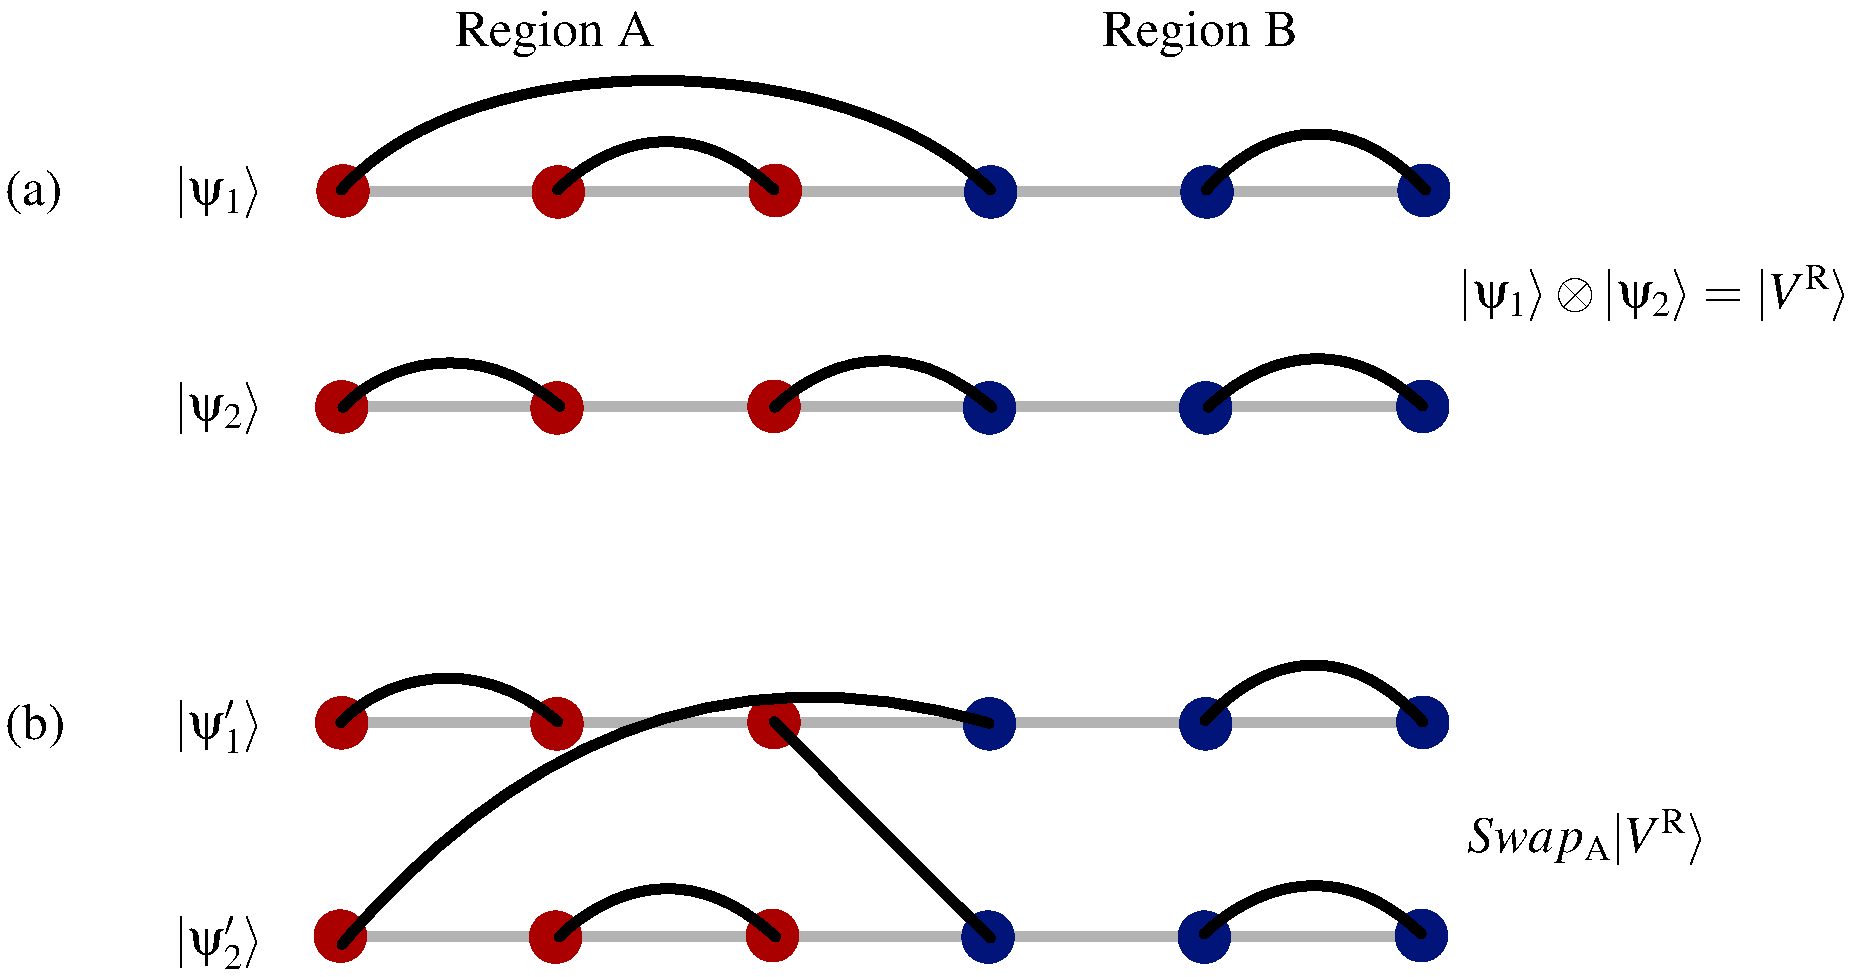
\includegraphics[width=6.2 in]{./figures/made/swp.pdf} 
	\caption[Application of the Swap operator]{
		\label{swap}
		(a) Two non-interacting copies, $\ket{\psi_1}$ and  $\ket{\psi_2}$, of a six-site chain
		where the left three sites of each copy belong to region A, and the other sites are in
		region B.
		
		(b) The same system from (a) after the $Swap_{\rm A}$ operator is applied.
		The endpoints of the valence bonds in region A are switched between copies 
		of the system.  Region B remains unswapped.
	}
}\end{figure}

The \swa operator acts on two copies of the system (see Figure \ref{swap}), where the copies are not necessarily in the same state.  The action of \swa is to exchange the configuration of region A, between the two copies of the system.  If region A has some entanglement with region B in one of both of the copies of the system, then the two copies will become entangled after the application of \swA.
The \swa operator can be more clearly defined in a basis such as the $S^z$ basis, in which an arbitrary state can be represented as a weighted sum of states decomposed into the separate a region A and a region B configuration.  
If we define $\{\ket{\alpha}\}$ as a complete basis of states spanning region A, and $\{\ket{\beta}\}$ as a complete basis of states spanning region B, then we can represent an arbitrary state as
\begin{equation}
	\ket{\psi} = \sum_{\alpha}\sum_{\beta} C_{\alpha,\beta}\ket{\alpha}\ket{\beta}
\end{equation}
for some set of coefficients $C_{\alpha,\beta}$.  
Then the effect of \swa on a two general states, $\ket{\psi_1}$ and $\ket{\psi_2}$ representing the two copies of the system, is
\begin{align}
	\SWA \ket{\psi_1} \otimes \ket{\psi_2}  &= 
		\SWA \left(\sum_{\alpha_1,\beta_1} 
		C_{\alpha_1,\beta_1}\ket{\alpha_1}\ket{\beta_1}\right) \otimes
			\left(\sum_{\alpha_2,\beta_2} 
		C_{\alpha_2,\beta_2}\ket{\alpha_2}\ket{\beta_2}\right) \\
			&=\sum_{\alpha_1,\beta_1}C_{\alpha_1,\beta_1}\sum_{\alpha_2,\beta_2} 
			C_{\alpha_2,\beta_2}
			\big(\ket{\alpha_2}\ket{\beta_1}\big)\otimes\big(\ket{\alpha_1}\ket{\beta_2}\big).
\end{align}
And the expectation value of \swa acting on two non-interacting copies of the ground state will be
\begin{align}
\langle \SWA \rangle &=
\bra{\Psi_0\otimes\Psi_0}\SWA \ket{\Psi_0\otimes\Psi_0} \\ 
	&=\sum_{\alpha_1,\beta_1} \sum_{\alpha_2,\beta_2}
		\overline{C}_{\alpha_2,\beta_1}C_{\alpha_1,\beta_1}
		\overline{C}_{\alpha_1,\beta_2}C_{\alpha_2,\beta_2}\\
	&=\sum_{\alpha_1,\alpha_2} \bra{\alpha_1}\rho_{\rm A} \ket{\alpha_2} 
					\bra{\alpha_2}\rho_{\rm A} \ket{\alpha_1}\\
	&={\rm Tr (\rho_A^2)}.
\end{align}
For more detail see Appendix \ref{swaperator}.  From Equation \eqref{renyi} the second Renyi entanglement entropy is
\begin{equation}
	S_2(\rho_{\rm A}) = -\ln\!\left[{\rm Tr}(\rho_{\rm A}^2)\right] = -\ln\left( \langle \SWA \rangle \right), \label{swapspectation}
\end{equation}
independent of basis.  Specifically, we can use \eqref{swapspectation} in the valence bond basis, where the \swa operator acts to swap the endpoints of valence bonds within region A between copies of the system, as in Figure \ref{swap}.

%----------------------------------------------------------------------------------------------------------
\subsection{Measuring the Swap Operator}
%----------------------------------------------------------------------------------------------------------

Since we are using the double projector algorithm for these measurements (Section \ref{sec:dubproj}) we use equations \eqref{generalop1} and \eqref{generalop2} to measure the \swa operator,
\begin{equation}
\langle \SWA \rangle = 
 \frac{   \sum_{l,r} W^L_l W^R_r  \bra{V^L_l} V^R_r\rangle    
		\frac{   \bra{V^L_l} \SWA  \ket{V^R_r}  }{   \bra{V^L_l} V^R_r\rangle  }}
							{\sum_{l,r} W^L_l W_r^R \bra{V^L_l} V^R_r\rangle}
	= \left<
		\frac{   \bra{V^L} \SWA \ket{V^R}  }{   \bra{V^L} V^R\rangle  }
						\right>,
\label{swapmeas}
\end{equation}
though in this case $\ket{V^{\rm L}}$ and $\ket{V^{\rm R}}$ each contain two non-interacting copies of the system we want to study, depicted in Fig.~\ref{swap}.


%----------------------------------------------------------------------------------------------------------
\section{1D Results}
%----------------------------------------------------------------------------------------------------------
We begin by measuring $S_2$ for a 1D OBC chain of length $L=100$, using the expectation value of the $Swap_x$ operator to find $S_2$ in VB QMC, where $x$ is the number of sites included in region A. 
The trial state $\ket{V}$ used is a simple dimerized state with only nearest neighbor valence bonds.
Results are shown in Figure \ref{swapfig}.
In the DMRG simulations, $S_2$ is calculated in the standard way, using the eigenvalues of the reduced density matrix. 
One can immediately see that the calculation of $S_2$ via the expectation value $\langle \SWA \rangle$ gives very large statistical errors, especially for a large number of sites inside region A.


\begin{figure} {
	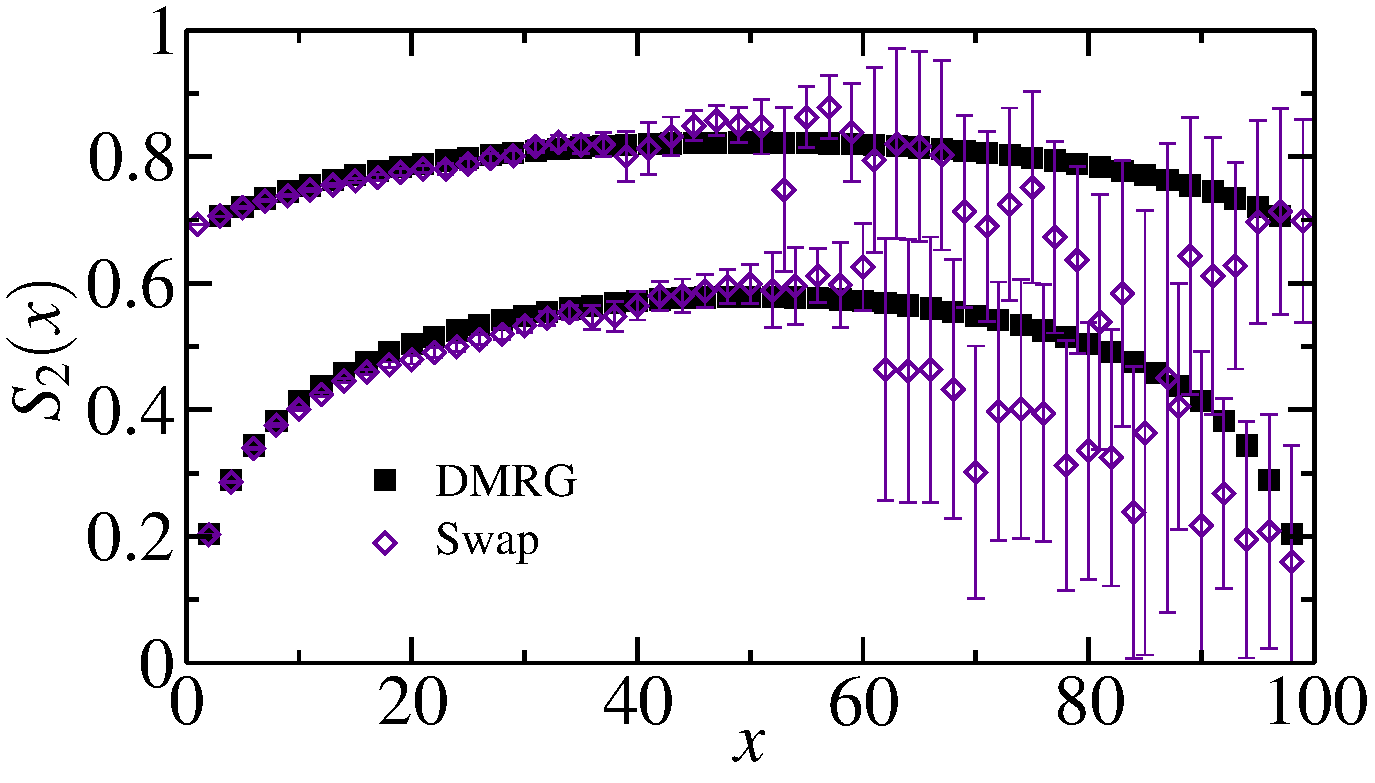
\includegraphics[width=6in]{./figures/paper2/fig_1D/swapfig.pdf} 
	\centering
	\caption[Renyi for 100 site chain]{ 
	\label{swapfig}
	The Renyi entropy $S_2$ as a function of site index $x \in $ A, for a 100-site Heisenberg chain with open boundaries, 
		calculated with DMRG and VB QMC.  Data labeled ``Swap'' was calculated with Eq.~\eqref{swapmeas} with one VB QMC simulation.	
	}
}\end{figure}

\begin{figure} {
	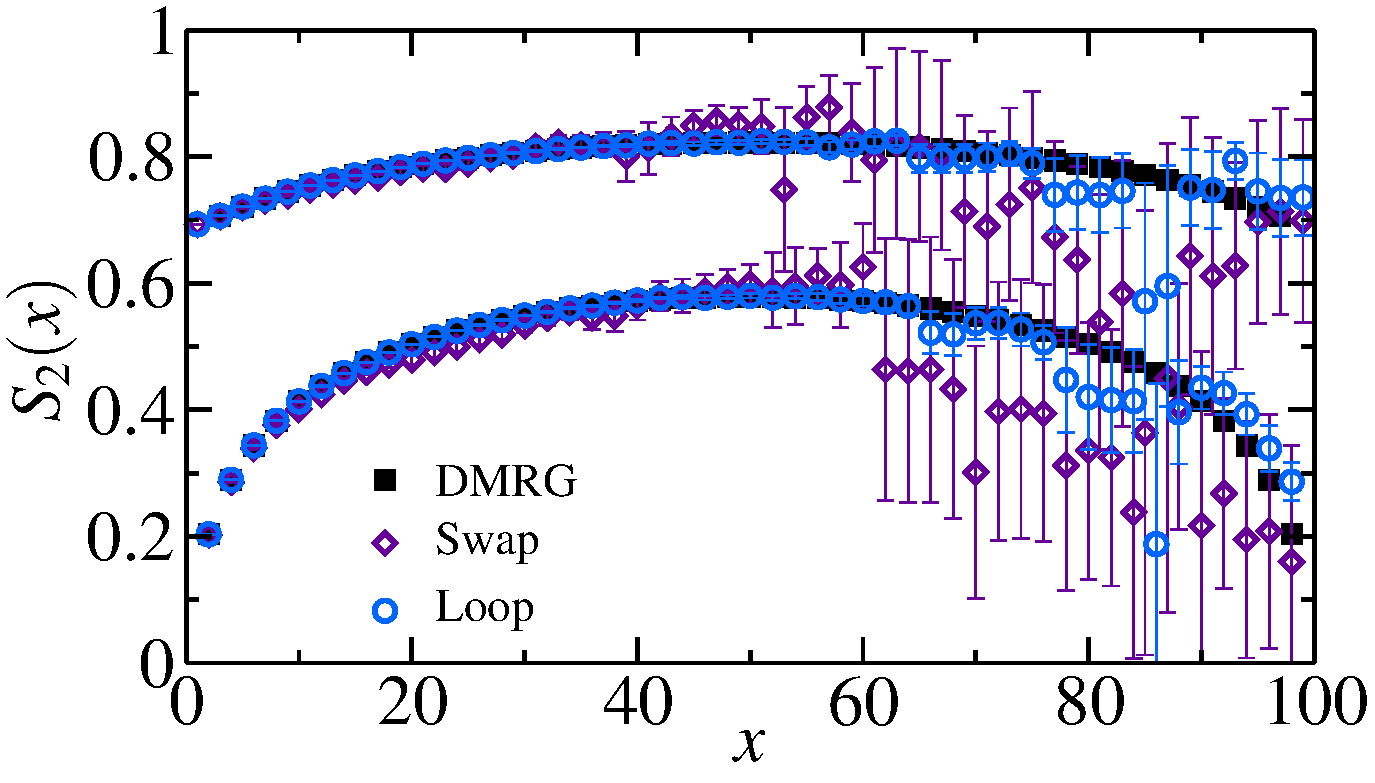
\includegraphics[width=6in]{./figures/paper2/fig_1D/loopfig.pdf} 
	\centering
	\caption[Renyi for 100 site chain]{ 
	\label{loopfig}
		hjk	
	}
}\end{figure}


	

%----------------------------------------------------------------------------------------------------------
\section{The ``Ratio Trick"}
%----------------------------------------------------------------------------------------------------------

\begin{equation}
\frac{\langle Swap_{i+j}\rangle}{\langle Swap_{i}\rangle} = 
\frac{ \sum_{l,r} W^L_l W^R_r \bra{V^L_l}Swap_{i+j} \ket{V^R_r}}
							{\sum_{l,r} W^L_l W_r^R \bra{V^L_l} Swap_i \ket{ V^R_r}}
\end{equation}

Instead of the weight from \eqref{supaweight}, the new weight is given by
\begin{equation}
W_{\rm total} = W^LW^R\bra{V^L} Swap_i \ket{V^R}
\end{equation}

\comment{make a diagram for this part of how the ratio stuff works.}

\begin{figure} {
	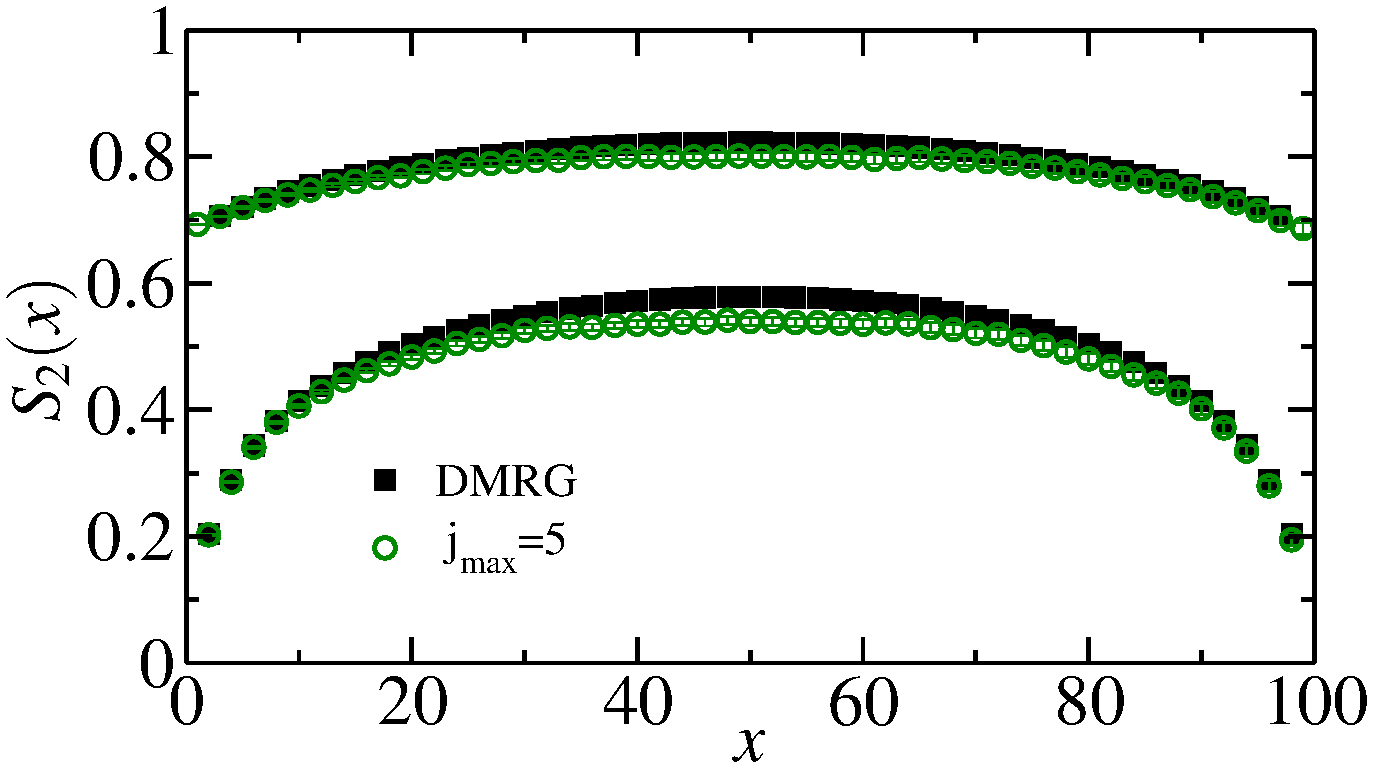
\includegraphics[width=6in]{./figures/paper2/fig_1D/ratiofig.pdf} 
	\centering
	\caption[Renyi for 100 site chain]{ 
	\label{ratiofig}
		, while
		data labeled $j_{\rm max}=5$ was calculated with Eq.~eqref{Ratio} using 20 separate QMC simulations with a range of  $j \in [1,5]$.  The inset shows the convergence of $S_2$ to the exact value (dashed line) for $i=6$ with up to $m=4000$.	
	}
}\end{figure}


%----------------------------------------------------------------------------------------------------------
\section{2D Results}
%----------------------------------------------------------------------------------------------------------

\begin{figure} {
	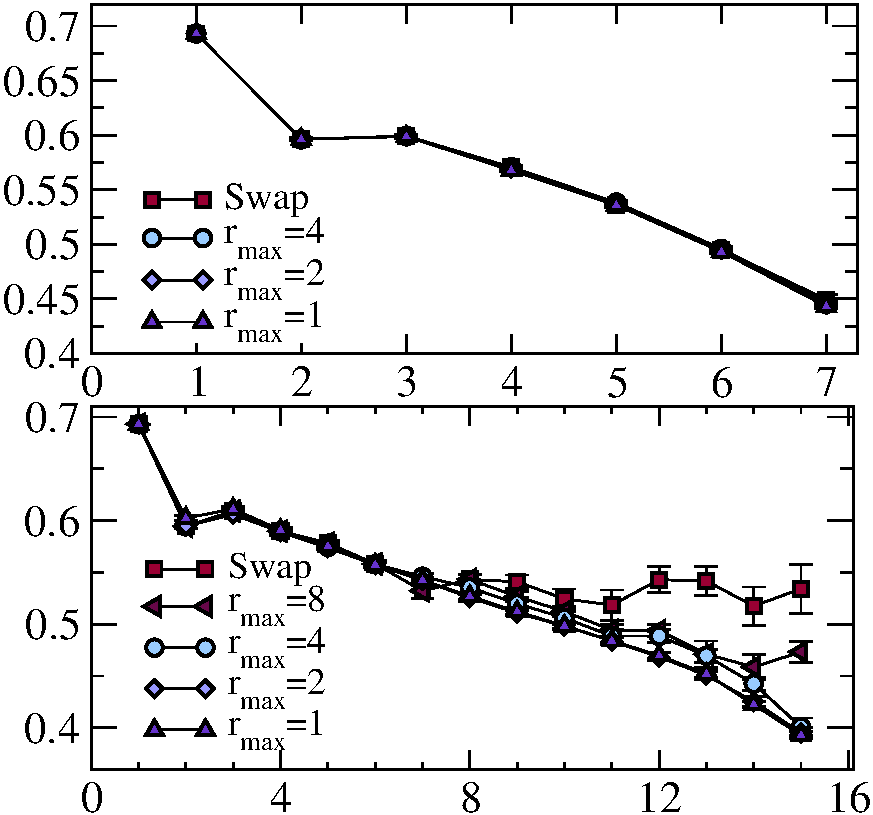
\includegraphics[width=5in]{./figures/paper2/fig_2DA/fig_L8n16.pdf} 
	\centering
	\caption[fds]{ fds
	\label{2Dfig}
	}
} \end{figure}

%----------------------------------------------------------------------------------------------------------
\section{The Area Law}
%----------------------------------------------------------------------------------------------------------

\begin{figure} {
	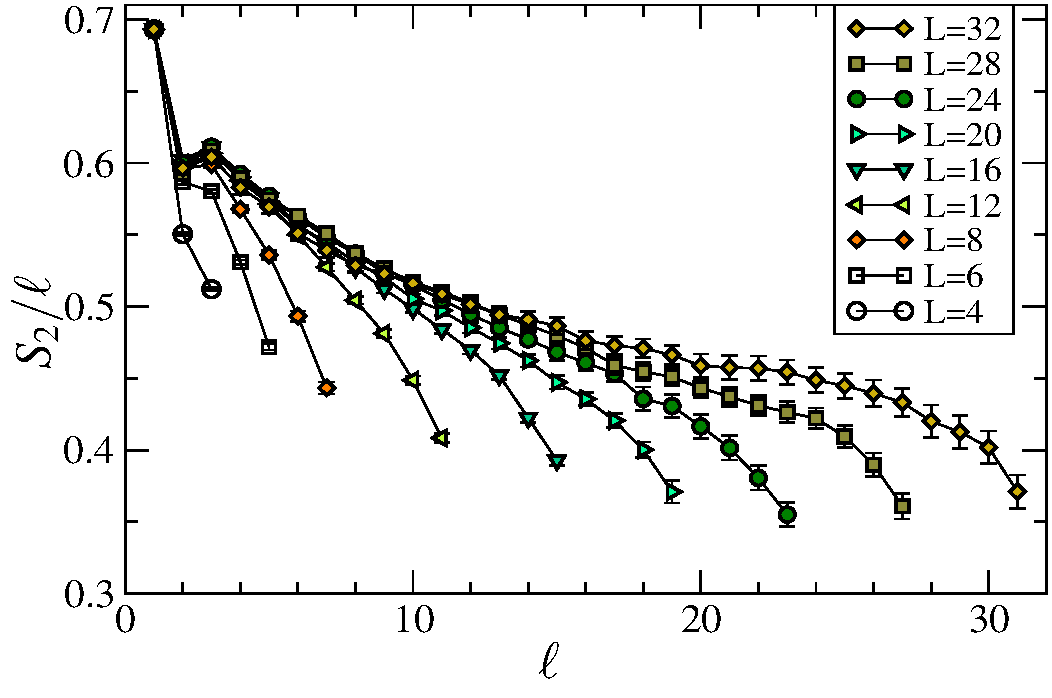
\includegraphics[width=5in]{./figures/paper2/fig_AreaL/fig4.pdf} 
	\centering
	\caption[fds]{ fds
	\label{2Dfig}
	}
} \end{figure}

\begin{figure} {
	\centering
	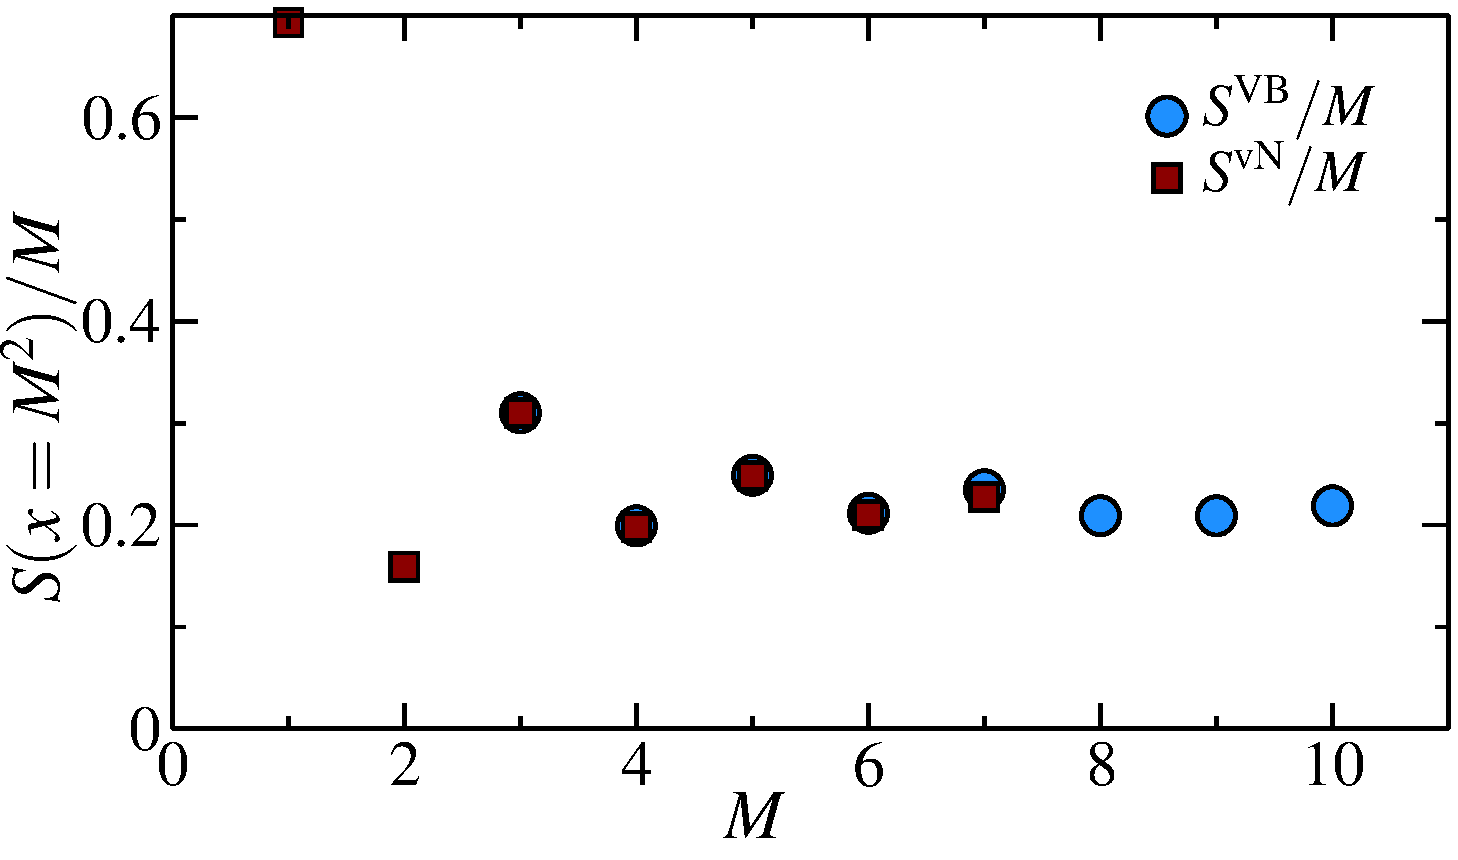
\includegraphics[width=5in]{./figures/made/marea.pdf} 
	\caption[fds]{ Add different cuts
	\label{2Dbetter}
	}
} \end{figure}
